\documentclass[10pt,a4paper]{book}
\usepackage[utf8]{inputenc}
\usepackage[english]{babel}
\usepackage{amsmath}
\usepackage{amsfonts}
\usepackage{adjustbox}
\usepackage{stmaryrd}
\usepackage{amssymb}
\usepackage{wrapfig}
\usepackage{mathtools}
\usepackage{graphicx}
\usepackage{cancel}
\usepackage[left=2cm,right=2cm,top=2cm,bottom=2cm]{geometry}
\usepackage{physics}
\usepackage{multicol}
\usepackage{caption}
\usepackage{subcaption}
\usepackage{amsmath}
\usepackage{amsfonts}
\usepackage{amssymb}
\usepackage{amsthm}
\usepackage{mathtools}
\usepackage{stmaryrd}
\usepackage[left=2cm,right=2cm,top=2cm,bottom=2cm]{geometry}


\author{Alessandro Pacco}
\title{Optics}
 

\newtheorem{thm}{Theorem}
\newtheorem{ex}{Example}
\newtheorem{definition}{Definition}

\begin{document}
\maketitle


\tableofcontents


\chapter{Classical description (in plane wave) of the field}
\section{Structure of the field}

We suppose that we have well collimated beams that propagate along an axis $\Rightarrow$ we can describe them as plane waves in first approximation. We will call $\vec{E}$ the electric field: 
$$\vec{E}(x,y,z,t)=E_0\vec{\epsilon}\cos(\omega t-n\vec{k}\cdot \vec{r}+\phi)$$
where $E_0$ is the amplitude (V/m), we will also express $E_0^2$ in watts; $\vec{\epsilon}$ is the polarisation; $\omega =2\pi\nu$; $\vec{k}$ is the wave vector with modulus given by $k=2\pi/\lambda$; $n$ is the optical index (1 in empty space); $\phi$ is the phase at the origin.
From now on we will write $\vec{k}=k\vec{e}_z$; $E_0\cos(\omega t-n\vec{k}\cdot \vec{r}+\phi)=\text{Re}(\epsilon_0e^{i(\omega t-n\vec{k}\cdot\vec{r})})$.
\section{Polarisation}
\subsection{General case of elliptical polarisation}
Recall that Maxwell's eq $\Rightarrow$ $\vec{k}\perp \vec{\epsilon}$, where $\vec{\epsilon}$ belongs to a 2 dim. vector space. $(\vec{k},\omega)\Rightarrow$ 2 possible polarisations. We have:
$$\vec{\epsilon}=\epsilon_x e^{i\phi_x}\vec{e}_x+\epsilon_y e^{i\phi_y}\vec{e}_y$$
and with $\epsilon_x,\epsilon_y\in\mathbb{R}^{*}$, $\phi_x=0$, it follows $$\vec{\epsilon}=\epsilon_x\bigg(\vec{e}_x+\vec{e}_y\frac{\epsilon_y}{\epsilon_x} e^{i\phi_y}\bigg)\Rightarrow \vec{E}(z=0,t)=E_0\epsilon_x\text{Re}\bigg((\vec{e}_x+\frac{\epsilon_y}{\epsilon_x}\vec{e}_ye^{i\phi_y})e^{i\omega t}\bigg)=E_0\epsilon_x\bigg(\cos\omega t\vec{e}_x+\frac{\epsilon_y}{\epsilon_x}\cos(\omega t+\phi_y)\vec{e}_y\bigg)$$

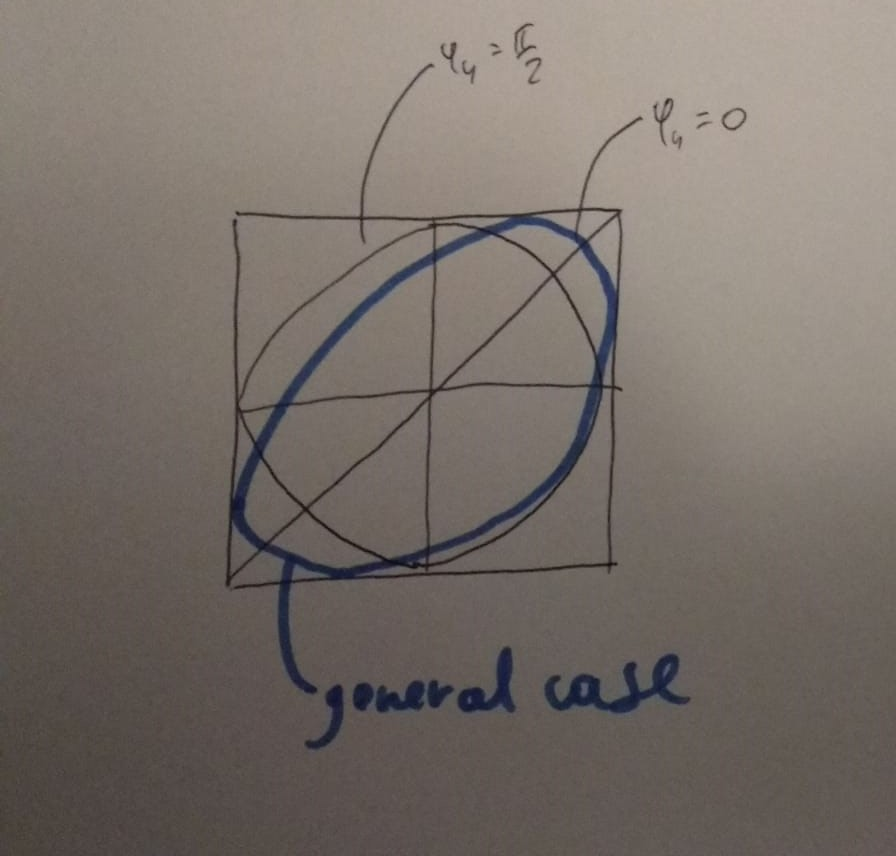
\includegraphics[scale=0.2]{fig1}
\subsection{Particular cases}
\subsubsection{Linear polarisation}
This is when $\phi_y-\phi_x=(0$ or $\pi)\Rightarrow \vec{E}(z=0,t)=E_0(\epsilon_x\vec{e}_x+\epsilon_y\vec{e}_y)\cos\omega t$
\subsubsection{Circular Polarisation}
We have
$$\begin{cases}
\phi_y-\phi_x=\pm\pi/2\\
\epsilon_x=\epsilon_y
\end{cases}\Rightarrow \vec{E}(z=0,t)=E_0(\vec{e}_x\cos\omega t\pm\vec{e}_y\sin\omega t)$$
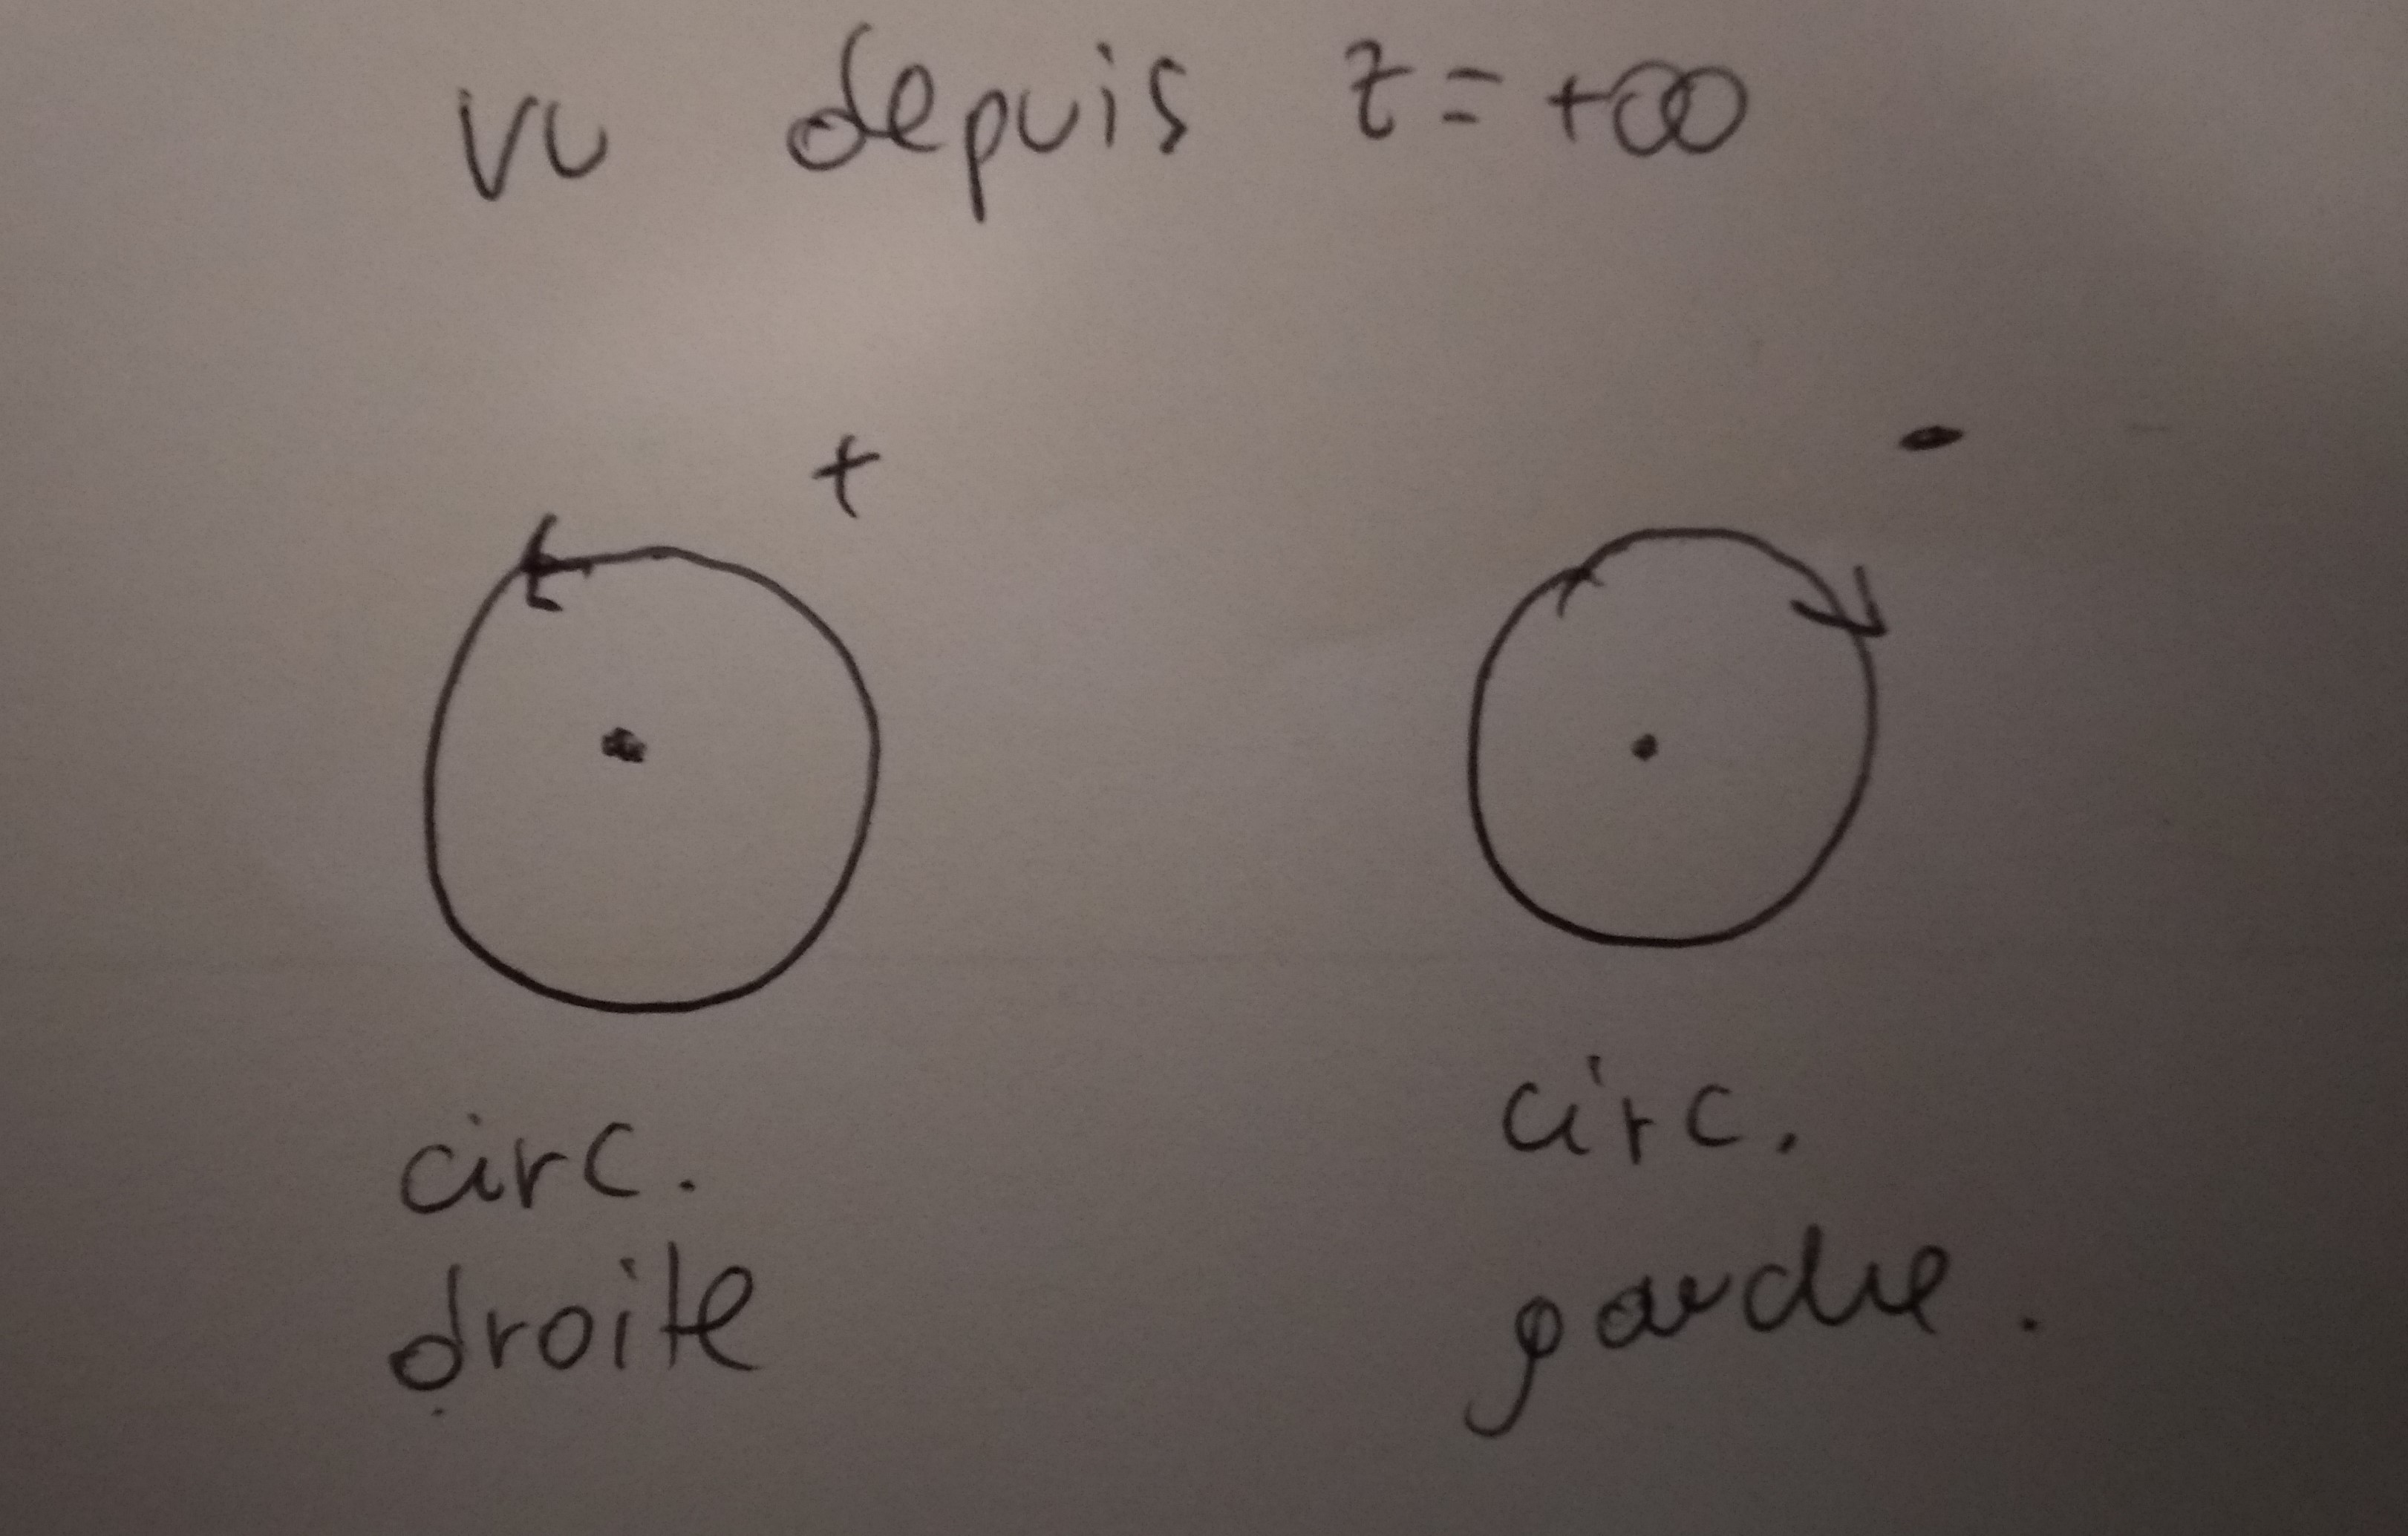
\includegraphics[scale=0.05]{fig2}

In atomic physics we care about the sense of circulation of the laser with respect to the atoms.
\subsection{Some optical components}
\subsubsection{Separation of polarisation cube}
Take a non isotropic material, $n$ depends on the polarisation $\Rightarrow$ if we consider a dioptre, the $R,T$ coefficients depend on the polarisation. [GRAPH]

\subsubsection{Wave blades}
Consider a material with $n_x,n_y$ that are different. Then consider $\vec{\epsilon}=\frac{1}{\sqrt{2}}(\vec{e}_x+\vec{e}_y)$ at $z=0$ and at $z=L$: $\vec{\epsilon}=\frac{1}{\sqrt{2}}(\vec{e}_xe^{-ikn_xL}+\vec{e}_ye^{-kn_yL})=\frac{1}{\sqrt{2}}e^{-ikn_xL}(\vec{e}_x+\vec{e}_ye^{-ik(n_y-n_x)L})$, then call $\Delta L=k(n_y-n_x)L$. Then we have the following:
\begin{align*}
k\Delta L&=0\quad \text{linear polarization}\\
k\Delta L&=\frac{\pi}{2}\quad \text{circulat polarization (gauche)}\\
k\Delta L&=\pi\quad \text{perpendicular polarization}\\
k\Delta L&=3\frac{\pi}{2}\quad \text{circular polarization (droite)} 
\end{align*}
Then we call quarter waveplate the component that changes the polarization so that $k\Delta L=0\to \frac{\pi}{2}$ and we call half waveplate the one that does $0\to \pi$.

\section{Modulations}
Take $\vec{E}=\text{Re}(E_0\vec{\epsilon}e^{i(kz-\omega t)})$[GRPAH]
\subsection{Phase modulation}
Take $E=E_0\text{exp}(i(\omega_0t+m\cos(\Omega t))=E_0e^{i\omega_0 t}(\sum_{k=-\infty}^{\infty} i^k J_k(m)e^{ik\Omega t})\approx E_0e^{i\omega_0 t}(1+i\frac{m}{2}(e^{i\Omega t}+e^{-i\Omega t}))$ for $m<<1$. In reality we get infinitely many terms expressed thanks to Bessel functions, but for $m<<1$ we maintain only the first 2 terms since the rest goes to zero. For small $m$ we have that apart from the main peak there are two smaller peaks that appear at same distance from the main one, one in the positive and the other in the negative part of the axis.
We have the following behaviors:\\\\
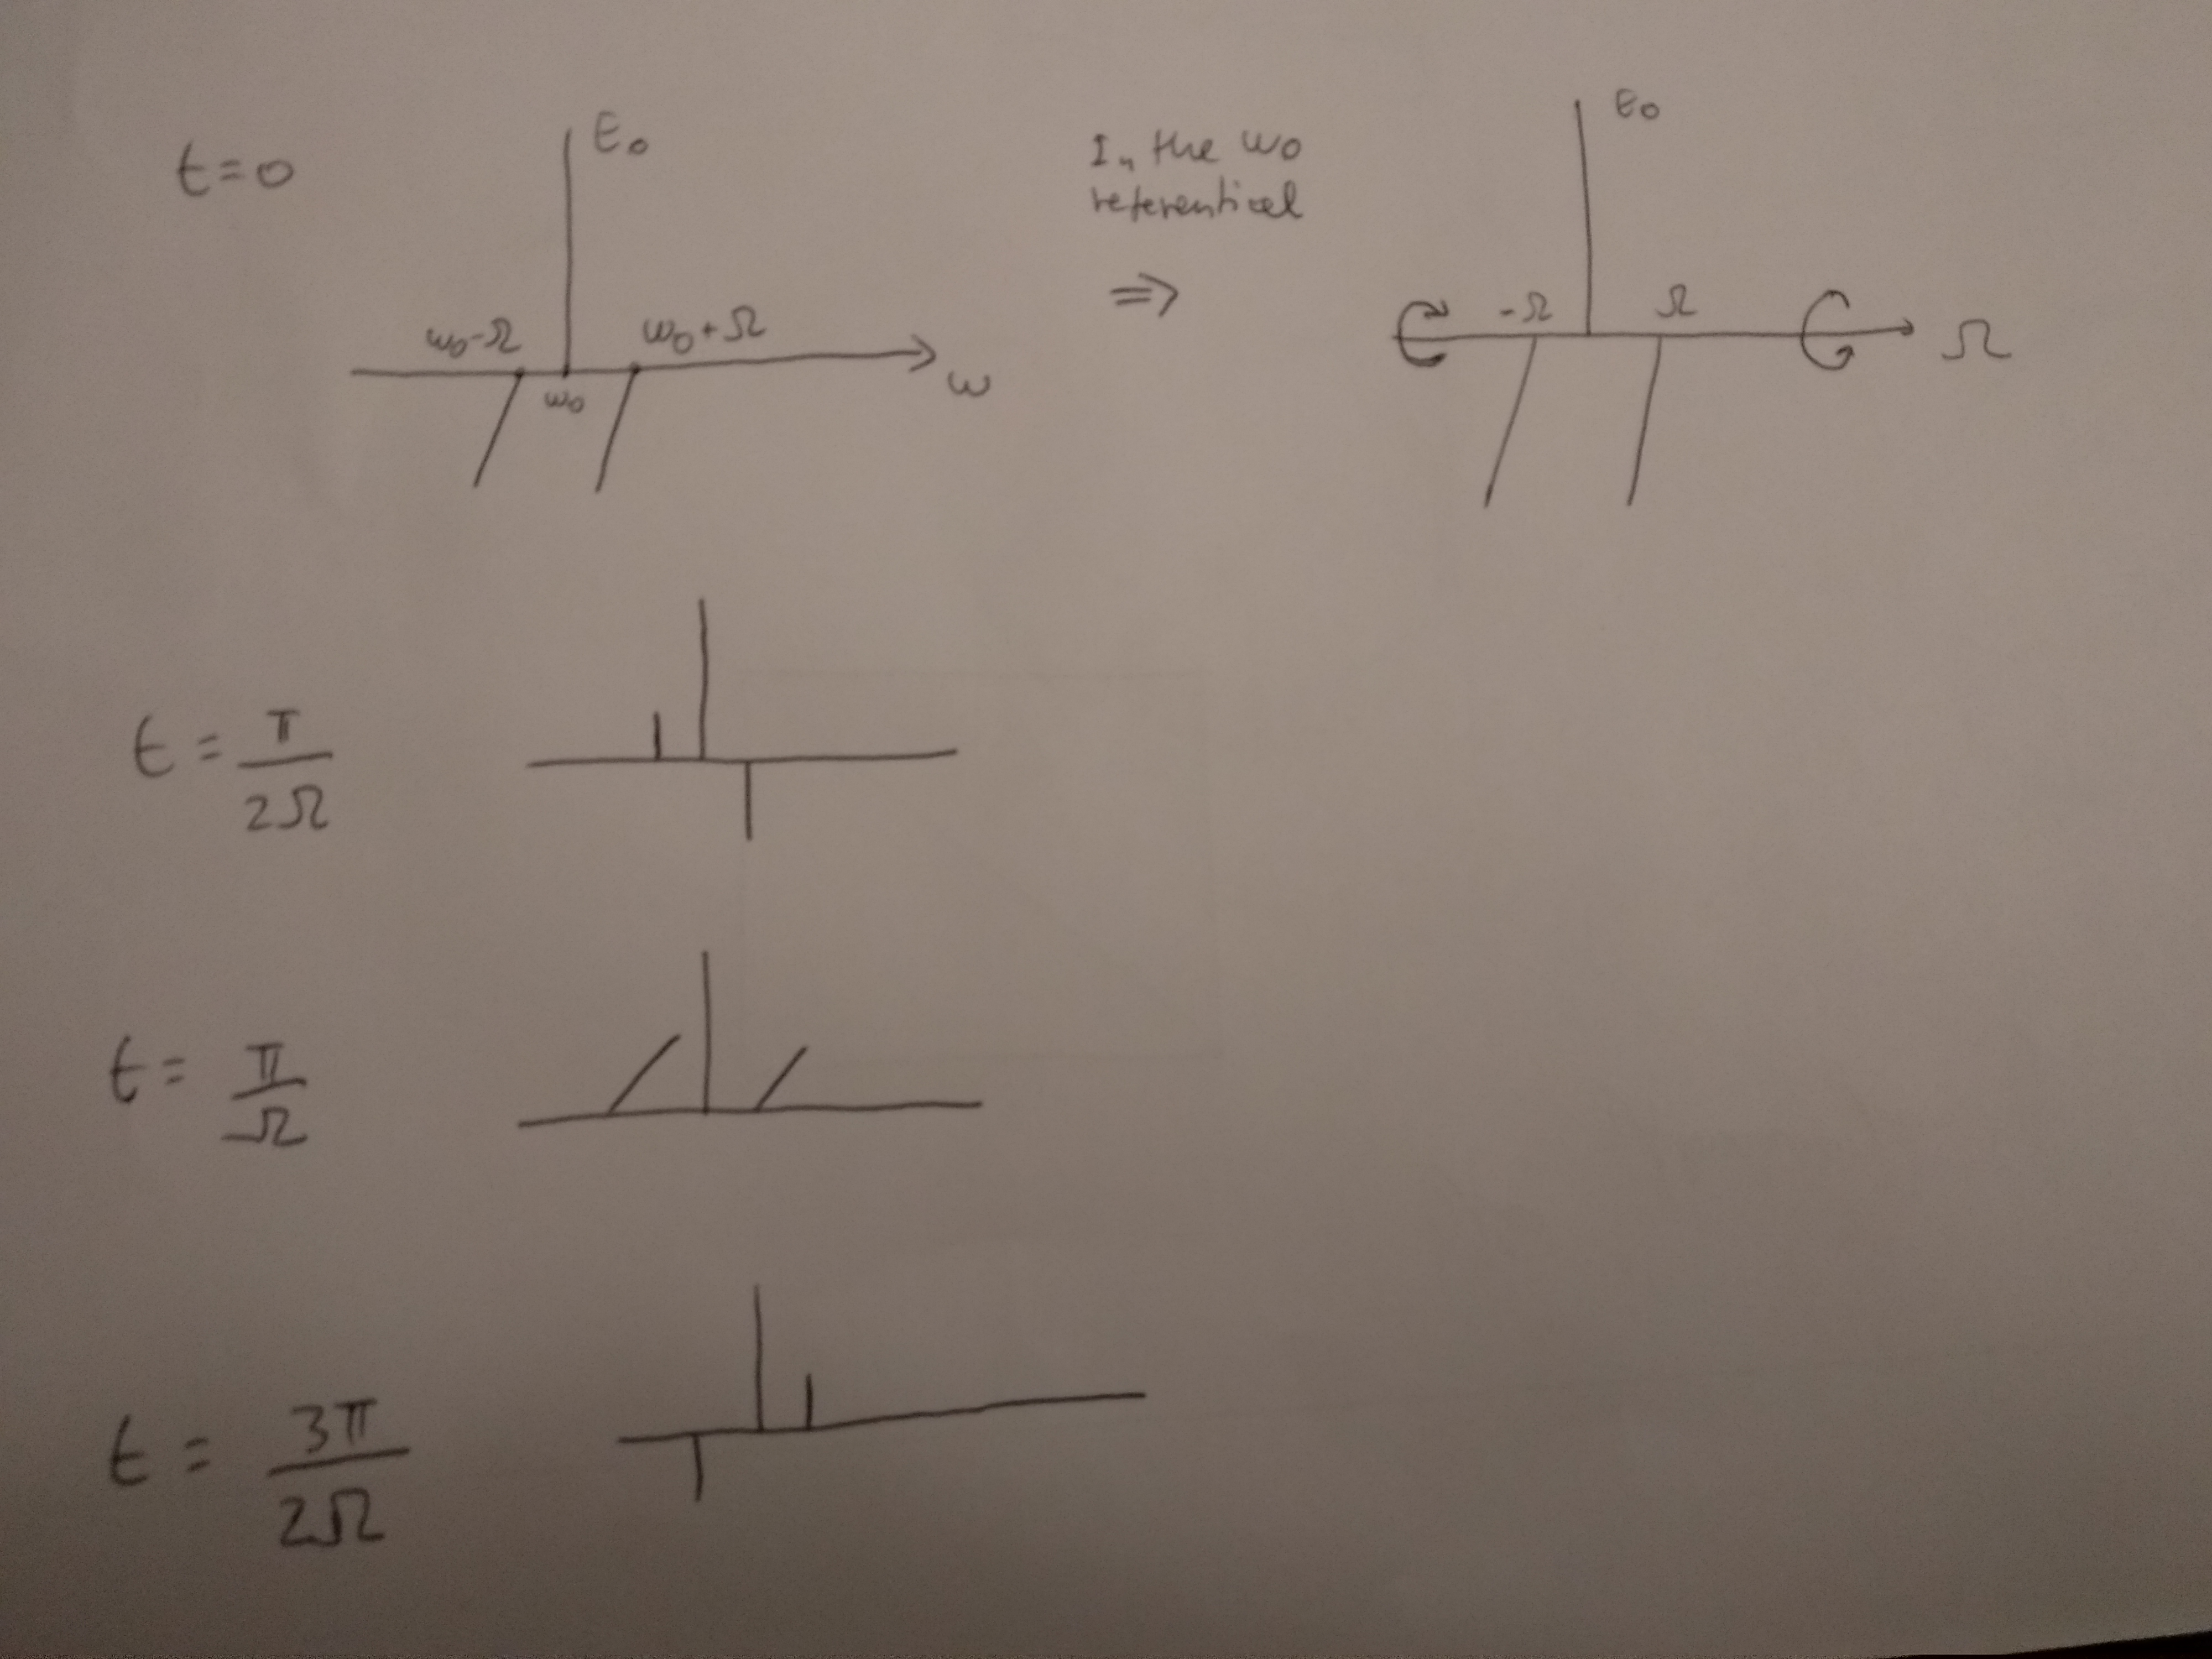
\includegraphics[scale=0.07]{fig3}\\\\
If instead $E=E_0(1+m\cos(\Omega t))e^{i\omega_0 t}=E_0(1+\frac{m}{2}(e^{i\Omega t}+e^{-i\Omega t}))e^{i\omega_0 t}$ we get:\\\\
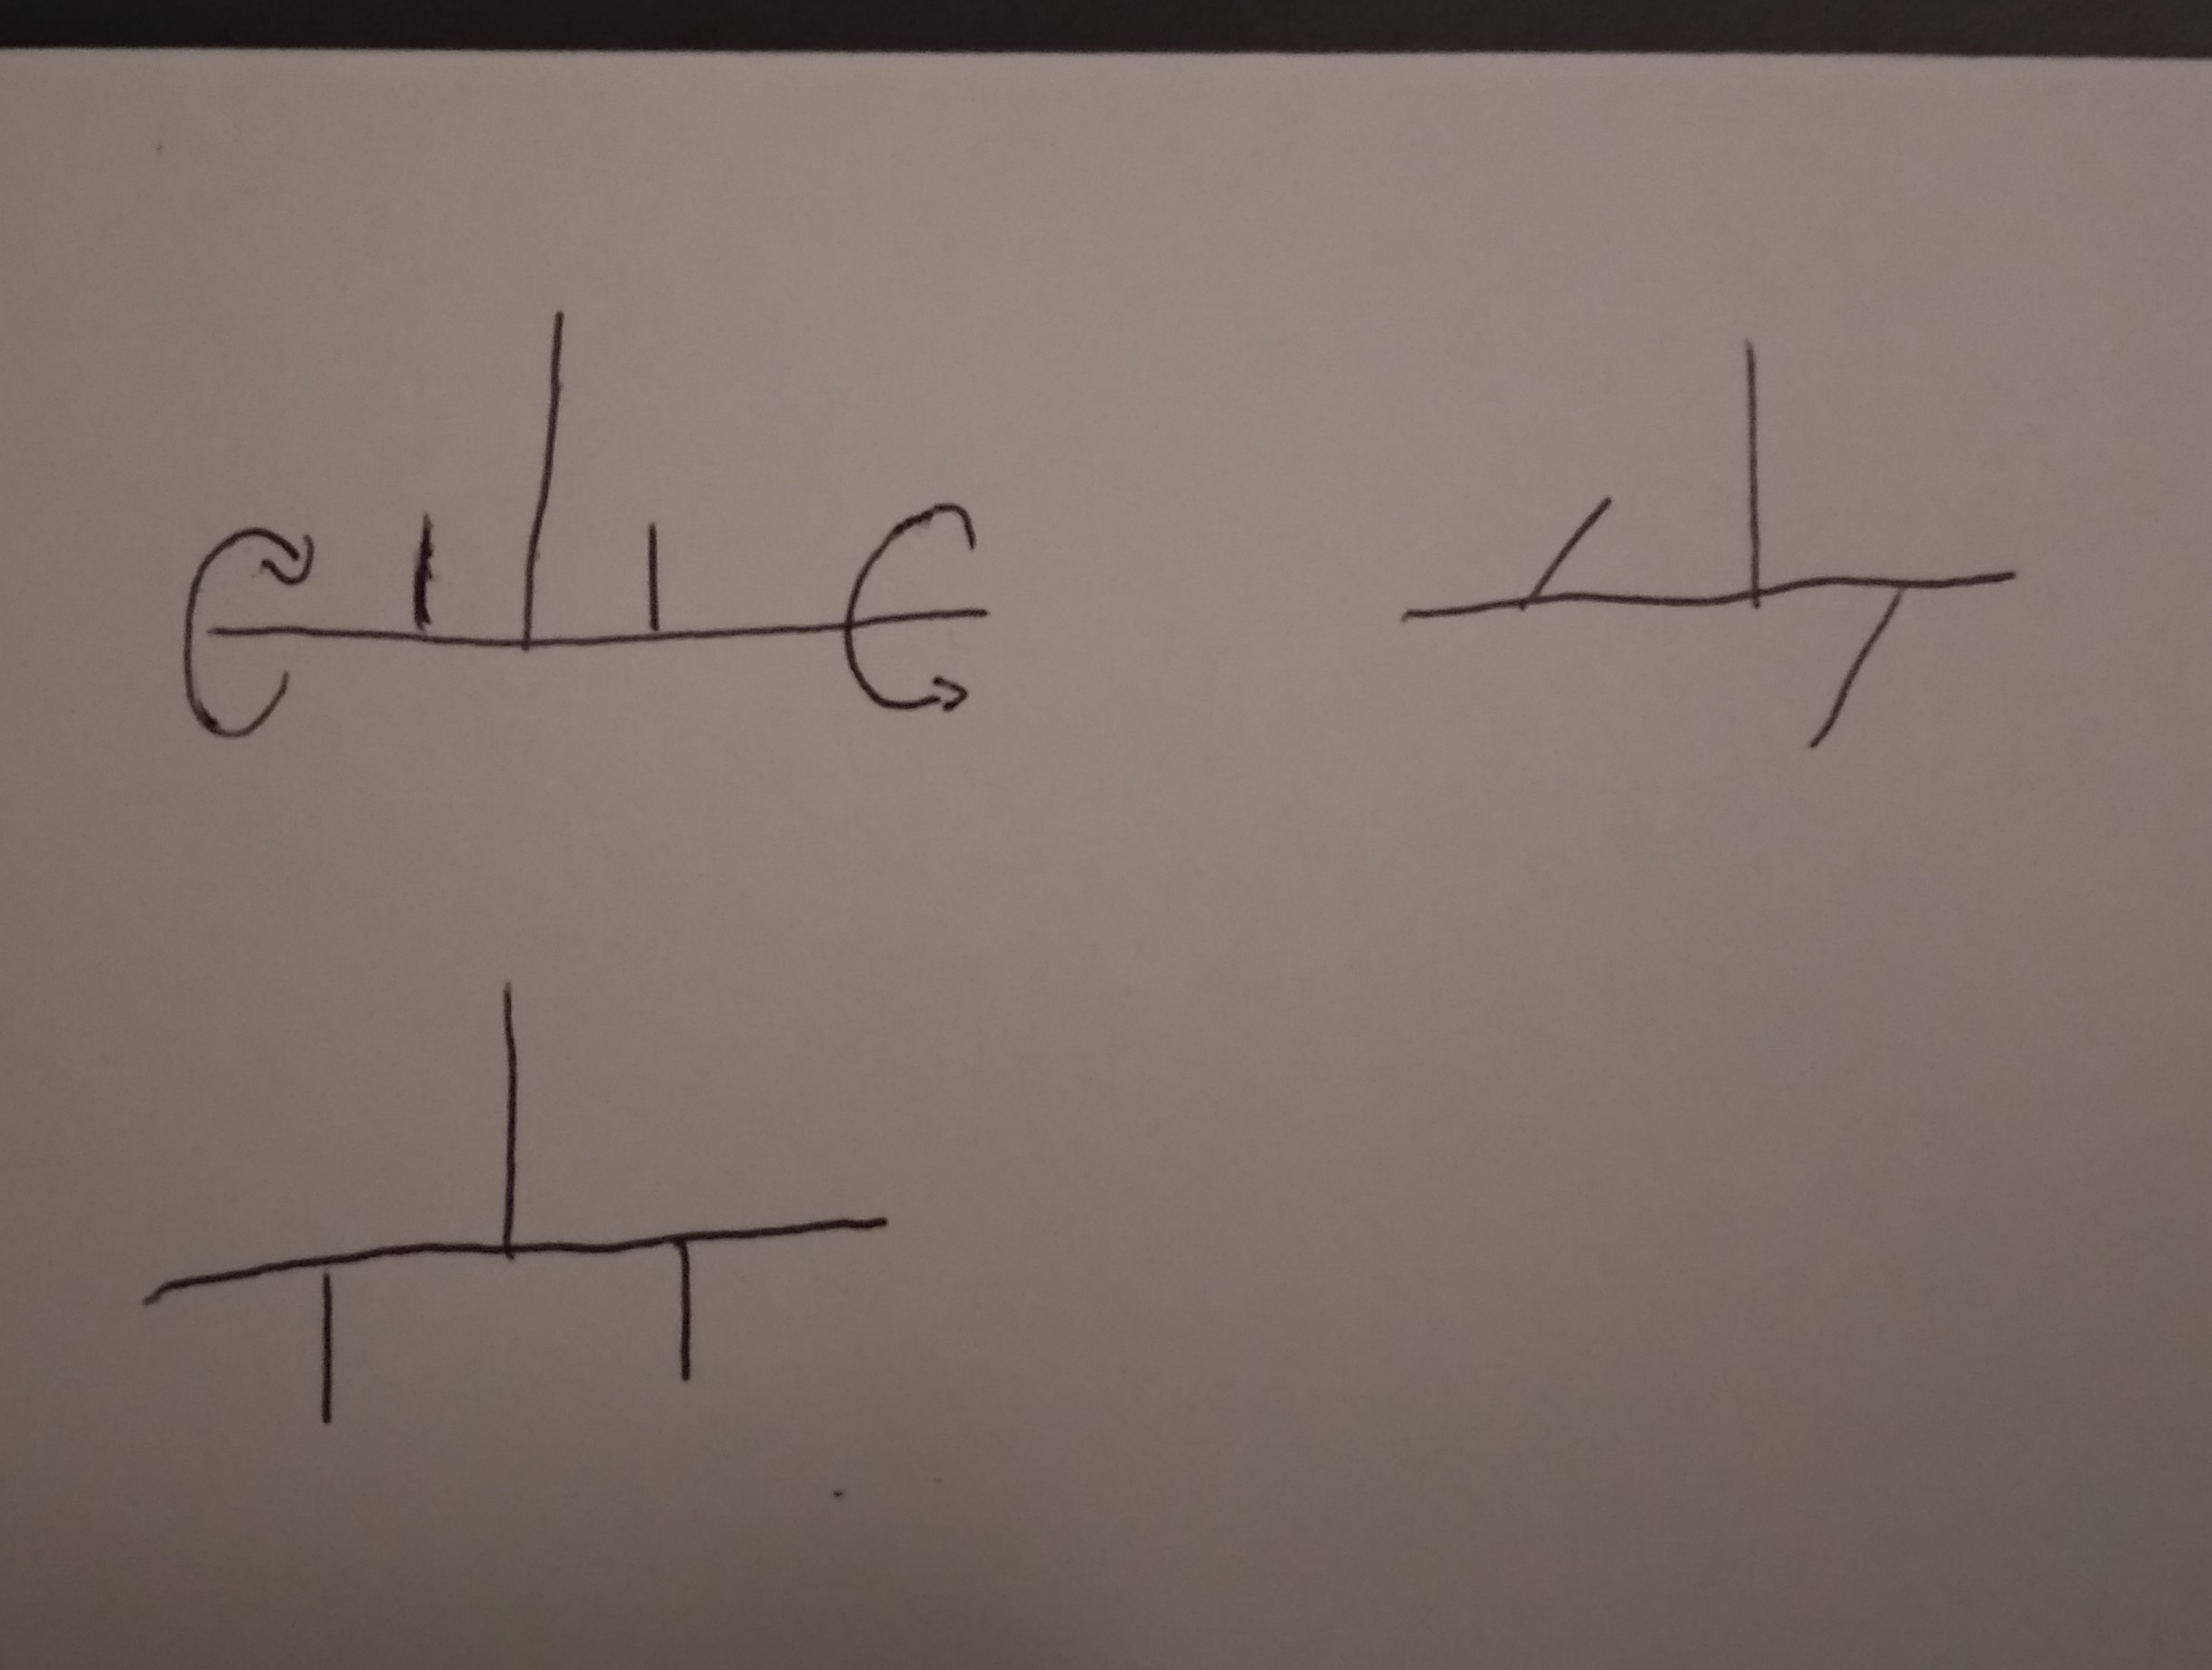
\includegraphics[scale=0.1]{fig4}\\\\
In conslusion modulated light has the main frequency and then the two modulated frequencies, which are one at right and the other at the left part of the first one. 

\chapter{Survey on the quantum description of light}
\section{Hamiltonian and field operator}
We forget about the polarisation and we say what is the Hamiltonian of the electromagnetic field. We place ourselves in a box. At each frequency there is an associated mode which is represented by an harmonic oscillator of the form $\epsilon_k(\frac{1}{2}m\omega_k^2x_k^2+\frac{p_k^2}{2m})$. The classical hamiltonian is
$$H=\int d^3r \frac{1}{2}\bigg(\epsilon_0E^2+\frac{B^2}{\mu_0}\bigg)$$
then the vector potential is written as 
$$\vec{A}=\epsilon_{\mu}\sqrt{\frac{\hbar}{2\epsilon_0L^3\omega_{\mu}}}\bigg(a_{\mu}\vec{e}_{\mu}+a^{\dagger}_{\mu}\vec{e}_{\mu}\bigg)$$
Increasing level in a harmonic oscillator is equivalent to absorbing at each step the same quantity of energy $\frac{\hbar\omega_0}{2}$ given by a photon with that particular energy. For one mode we have that the electric field opearator is $E=\sqrt{\frac{\hbar\omega_0}{2\epsilon_0L^3}}(a+a^{\dagger})$. That operator gives the maximum amplitude of the electric field for each mode.


\section{Effect of the quantum fluctuations of empty space}
On paper...






\end{document}